\documentclass[11pt,a4paper,twoside]{book}
\usepackage[margin=2.5cm]{geometry}
\usepackage{fontspec}
\usepackage{unicode-math}
\usepackage{microtype}
\usepackage{graphicx}
\usepackage{xcolor}
\usepackage{tikz}
\usepackage{tcolorbox}
\usepackage{fancyhdr}
\usepackage{lettrine}
\usepackage{yfonts}
\usepackage{hyperref}
\usepackage{soul}
\usepackage{contour}
\usepackage[strict]{changepage}
\usepackage{wrapfig}
\usepackage{multicol}
\usepackage{tabularx}
\usepackage{array}
\usepackage{pgfornament}
\usetikzlibrary{shapes,decorations.pathmorphing,shadows,patterns}

% Font setup for fantasy feel - using fallback fonts
\setmainfont{Latin Modern Roman}[
    Ligatures=TeX,
    Numbers=OldStyle
]
\newfontfamily\displayfont{Latin Modern Roman}[
    Ligatures=TeX,
    Scale=1.2
]
\newfontfamily\runefont{Latin Modern Roman}[
    Scale=1.1,
    FakeSlant=0.2
]

% Color definitions - transition from light to dark
\definecolor{dawn}{RGB}{255, 220, 150}
\definecolor{dusk}{RGB}{120, 80, 140}
\definecolor{blood}{RGB}{139, 0, 0}
\definecolor{void}{RGB}{20, 0, 30}
\definecolor{candlelight}{RGB}{255, 200, 100}
\definecolor{corruption}{RGB}{80, 20, 80}
\definecolor{parchment}{RGB}{253, 246, 227}
\definecolor{ink}{RGB}{40, 30, 20}
\definecolor{eldritchgreen}{RGB}{50, 120, 80}

% Page background
\pagecolor{parchment}
\color{ink}

% TColorBox styles for different game phases
\tcbset{
    heroicbox/.style={
        colback=dawn!10,
        colframe=dawn!80,
        arc=3mm,
        boxrule=2pt,
        fonttitle=\displayfont\large,
        drop lifted shadow,
        title={#1}
    },
    horrorbox/.style={
        colback=void!20,
        colframe=blood!80,
        arc=0mm,
        boxrule=3pt,
        fonttitle=\runefont\large,
        fuzzy shadow={2mm}{-2mm}{0mm}{0.5mm}{corruption},
        title={#1}
    },
    codexbox/.style={
        colback=parchment!90,
        colframe=ink!70,
        arc=2mm,
        boxrule=1.5pt,
        fonttitle=\displayfont\normalsize,
        coltitle=ink,
        attach boxed title to top left={yshift=-2mm,xshift=4mm},
        boxed title style={colback=parchment,boxrule=0.5pt,arc=1mm},
        title={#1}
    },
    itembox/.style={
        colback=candlelight!5,
        colframe=candlelight!60,
        arc=1mm,
        boxrule=1pt,
        fonttitle=\bfseries,
        title={#1}
    }
}

% Custom commands for text effects
\newcommand{\corrupt}[2]{%
    \contour{corruption}{#1}%
    \llap{\color{blood!30}#2}%
}

\newcommand{\fadetext}[1]{%
    \textcolor{ink!30}{#1}%
}

\newcommand{\glitch}[1]{%
    \textcolor{eldritchgreen!80}{\textit{#1}}%
}

% Header/footer styling
\pagestyle{fancy}
\fancyhf{}
\fancyhead[LE]{\small\textit{The Unraveling of Kándavael}}
\fancyhead[RO]{\small\textit{From Light to Dæl}}
\fancyfoot[C]{\thepage}
\renewcommand{\headrulewidth}{0.5pt}
\renewcommand{\footrulewidth}{0.5pt}

% Custom decoration commands
\newcommand{\fancybreak}{%
    \begin{center}
    \pgfornament[width=3cm]{88}
    \end{center}
}

\title{
    \displayfont\Huge
    The Unraveling of\\
    \vspace{0.5em}
    {\Huge K}\corrupt{á}{â}ndavael\\
    \vspace{1em}
    \large\textit{An Artbook of Linguistic Horror}\\
    \vspace{0.5em}
    \normalsize\textit{Where High Vaelic Bleeds into Under-Vêlth}
}
\author{
    \textit{A Complete Guide to the Realm's Descent}
}
\date{}

\begin{document}

\frontmatter
\maketitle

\chapter*{Content Warning}
\begin{adjustwidth}{2em}{2em}
\textit{This document contains descriptions of body horror, psychological manipulation, religious subversion, and linguistic corruption. The game explores themes of cosmic horror through the decay of language and meaning.}
\end{adjustwidth}

\tableofcontents

\mainmatter

\part{The Deception}

\chapter{Welcome to Kándavael}

\begin{wrapfigure}{r}{0.4\textwidth}
    \centering
    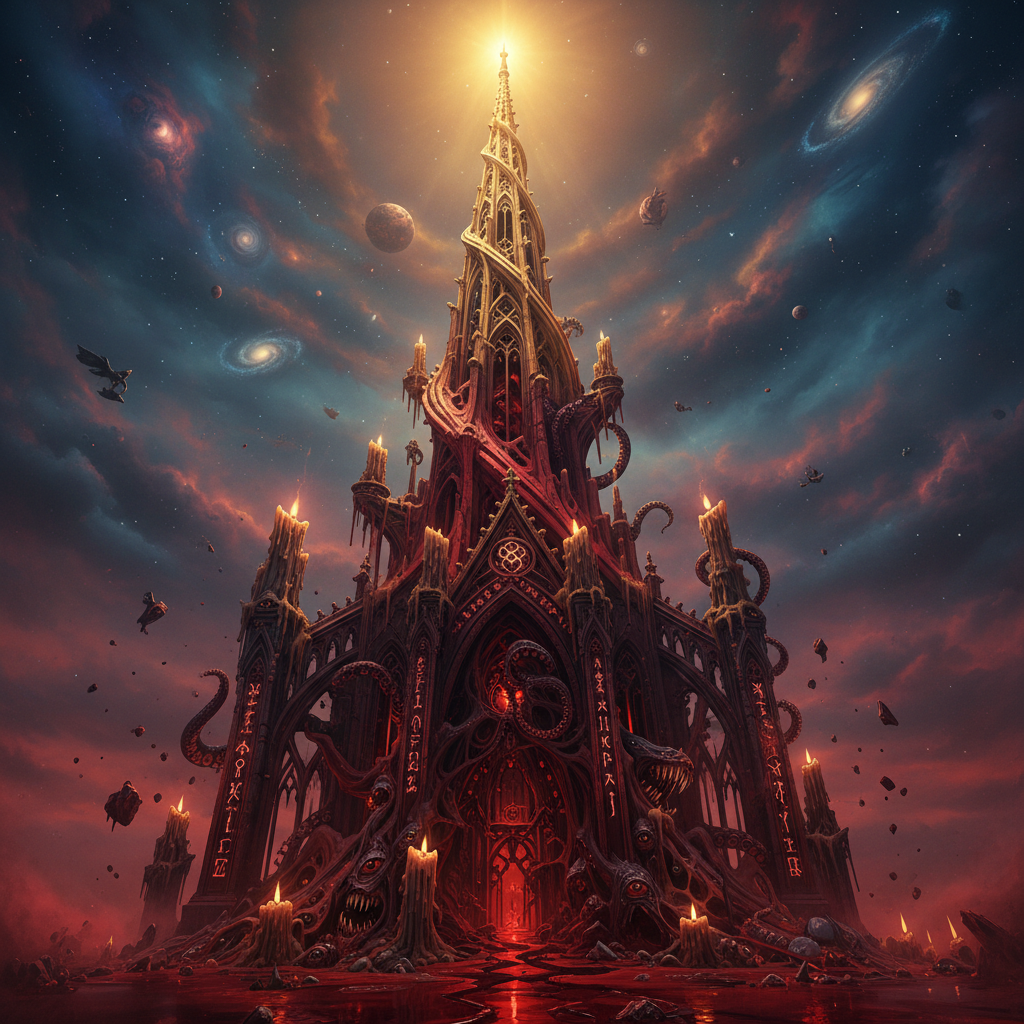
\includegraphics[width=0.35\textwidth]{images/daelspire_transformation_2025-09-03T22-21-48-135Z_1.png}
    \caption*{\small\textit{The Daelspire - beacon of hope}}
\end{wrapfigure}

\lettrine[lines=4]{\color{dawn}Y}{ou} have been summoned! Through prophetic visions and arcane ritual, the Court Wizard Alaric has reached across realities to find their Champion. You—yes, you from Earth—have been chosen by the benevolent \textit{Dael Tríthae} (Dawn Triumvirate) to save the prosperous kingdom of Kándavael from the lingering corruption of the tyrannical Dusk Rhael.

Villages celebrate your arrival with festivals of beeswax candles and honey wine. Children throw flower petals at your feet. The golden sun shines upon fertile fields, and hope returns to hearts long dimmed by the Dusk King's cruelty.

\begin{figure}[h]
\centering
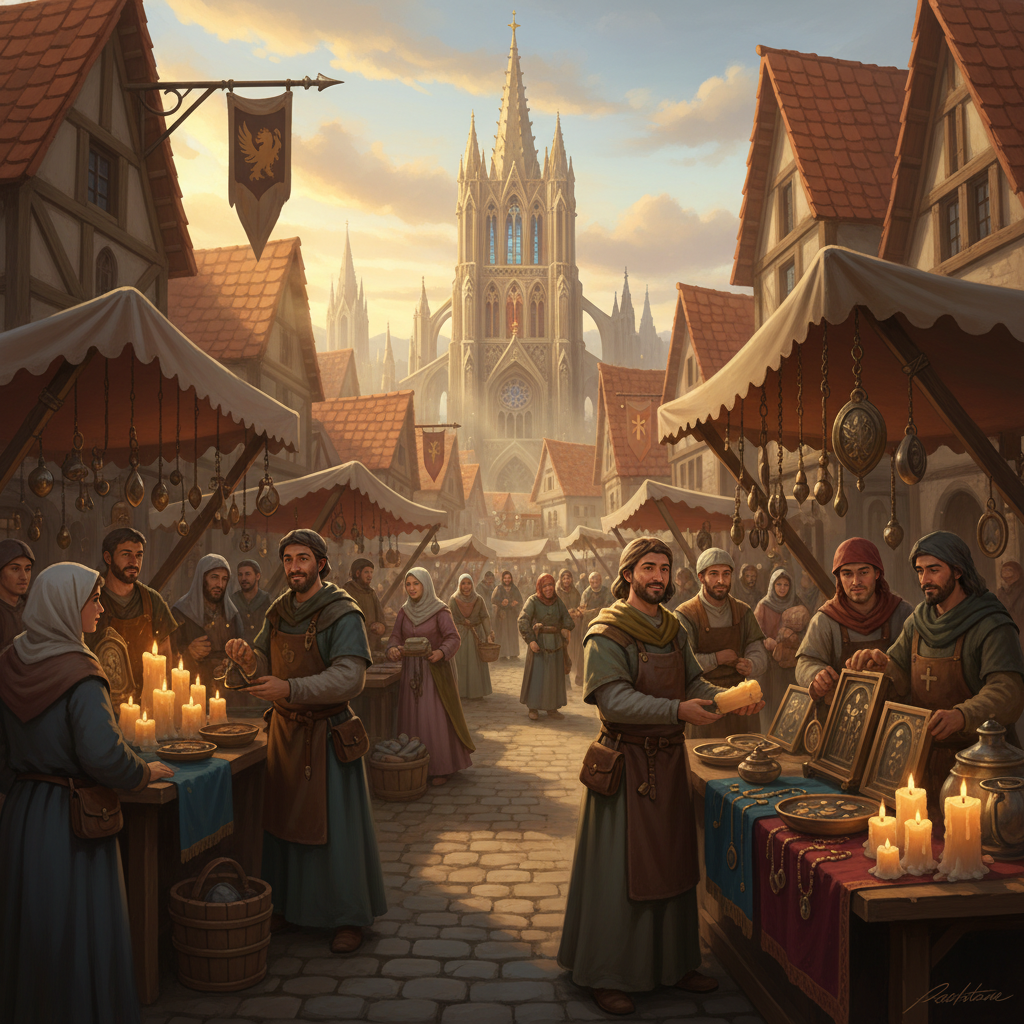
\includegraphics[width=0.8\textwidth]{images/market_dawn_2025-09-03T22-29-52-092Z_1.png}
\caption*{\textit{The prosperous markets of Kándavael at dawn}}
\end{figure}

\section{Your Noble Quest}

\begin{tcolorbox}[heroicbox={The Prophecy}]
\centering
\displayfont\large
"When shadows grow teeth and children sing again,\\
the Fall-born Champion shall kindle the Dawn"\\
\normalfont
\vspace{1em}
\textit{—Ancient prophecy of the Dael Tríthae}
\end{tcolorbox}

Your mission is clear and righteous:
\begin{itemize}
    \item Light the Four Beacons of Dawn to push back the darkness
    \item Defeat the Vardain, the Dusk King's cruel lieutenants  
    \item Sanctify corrupted shrines with blessed light
    \item Restore prosperity to Kándavael's villages
    \item Kindle the Last Lantern to banish evil forever
\end{itemize}

\fancybreak

\section{The Blessed Mechanics}

\subsection{The Trinity of Virtues}

Your power manifests through three divine meters:

\begin{center}
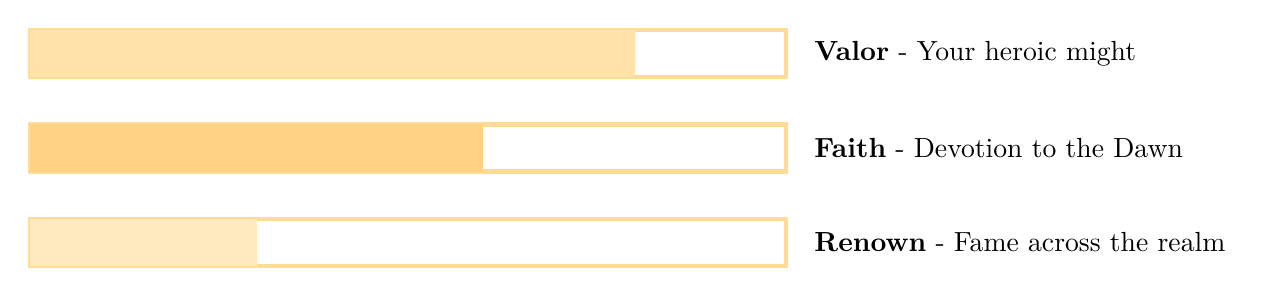
\begin{tikzpicture}[scale=1.2]
    % Valor meter
    \draw[dawn, ultra thick] (0,0) rectangle (8,0.5);
    \fill[dawn!80] (0,0) rectangle (6.4,0.5);
    \node[right] at (8.2,0.25) {\textbf{Valor} - Your heroic might};
    
    % Faith meter
    \draw[dawn, ultra thick] (0,-1) rectangle (8,-0.5);
    \fill[candlelight!80] (0,-1) rectangle (4.8,-0.5);
    \node[right] at (8.2,-0.75) {\textbf{Faith} - Devotion to the Dawn};
    
    % Renown meter
    \draw[dawn, ultra thick] (0,-2) rectangle (8,-1.5);
    \fill[dawn!60] (0,-2) rectangle (2.4,-1.5);
    \node[right] at (8.2,-1.75) {\textbf{Renown} - Fame across the realm};
\end{tikzpicture}
\end{center}

\subsection{Divine Prayer System}

The Dael Tríthae grant you holy words of power:

\begin{tcolorbox}[codexbox={Basic Prayers}]
\begin{tabular}{ll}
\textbf{LIGHT + WARD} & Creates protective aura \\
\textbf{HEAL + SELF} & Restores your vitality \\
\textbf{BLESS + BLADE} & Sanctifies your weapon \\
\textbf{DAWN + KINDLE} & Ignites sacred flames \\
\end{tabular}
\end{tcolorbox}

\chapter{The Land and Its People}

\section{Noble Settlements}

\subsection{Daelspire - The Radiant Capital}

\begin{tcolorbox}[heroicbox={Daelspire}]
\textit{"Where dawn never dies and candles burn eternal"}

The magnificent spire-city rises from morning mists, its towers catching first light like fingers of gold. Here, the Cathedral of First Dawn houses the sacred Beacon, and merchants trade in blessed beeswax worth its weight in silver.
\end{tcolorbox}

\textbf{Notable Features:}
\begin{itemize}
    \item The Everburning Chandeliers - lit since the kingdom's founding
    \item Academy of Divine Light - where priests learn the holy tongue
    \item The Honey Markets - sweetness flows like liquid gold
    \item Dawn Guard Barracks - protectors of the faithful
\end{itemize}

\subsection{Villages of the Vale}

\begin{multicols}{2}
\textbf{Lindenhael}\\
\textit{"The Healer's Haven"}\\
Famous for medicinal herbs and the Temple of Blessed Restoration. Elder Haelric teaches the youth old prayers and proper pronunciations.

\columnbreak

\textbf{Tríthbridge}\\
\textit{"Where Three Waters Meet"}\\
Built at the confluence of three pure rivers, blessed by the Trinity themselves. The bridges sing at dawn.
\end{multicols}

\section{Your Allies}

\begin{wrapfigure}{l}{0.45\textwidth}
    \centering
    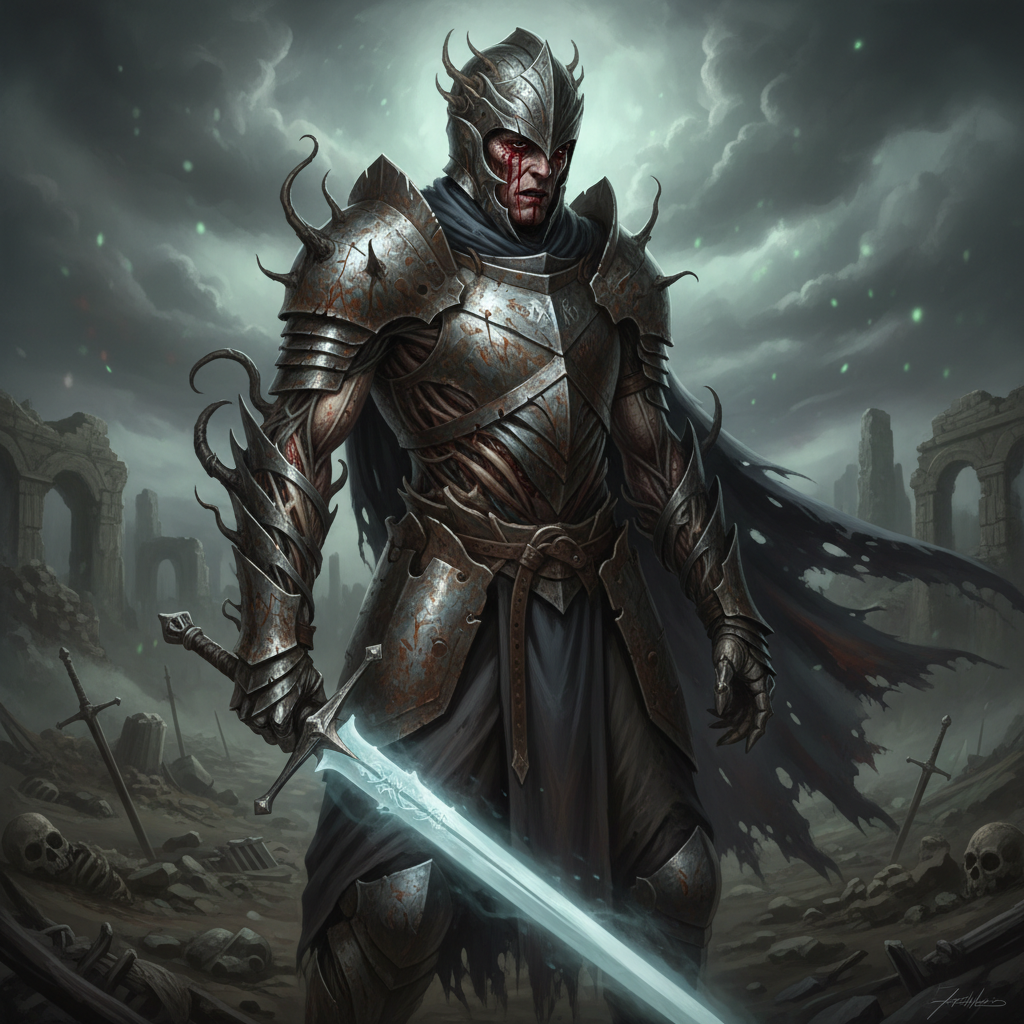
\includegraphics[width=0.4\textwidth]{images/candle_knight_2025-09-03T22-23-00-355Z_1.png}
    \caption*{\small\textit{Sir Gareth of the Candle Knights}}
\end{wrapfigure}

\subsection{Priestess Ael-Saelána}

Your primary guide and mentor, Ael-Saelána serves as High Priestess of the Dawn Triumvirate. Her warm smile and healing hands have comforted countless souls. She provides you with blessed items and teaches you the prayers needed for your quest.

\textit{"Welcome, Champion! The Dawn has smiled upon us with your arrival. Come, let me teach you our sacred words..."}

\subsection{Captain Líndrel}

A veteran of the wars against the Dusk King, Captain Líndrel trains you in combat. His family medallion bears the old seal of valor, passed down through seven generations of service.

\textit{"Hold your blade steady, Champion. The darkness tests our resolve, but dawn always follows night."}

\subsection{The Candle Knights}

An order of paladins sworn to protect the innocent, their blessed armor never tarnishes and their faith never wavers. They patrol the roads, keeping travelers safe from bandits and monsters.

\fancybreak

\part{The Unraveling}

\chapter{When Language Bleeds}

\lettrine[lines=4]{\color{dusk}A}{round} Floor 10, something shifts. Not dramatically—subtly. A village elder pronounces "Kándavael" as "Khândavêl." You correct them. They smile sadly and nod, but their lips still shape the darker sounds. 

The merchant's "blessed candles" sound like "bled candles" in his thick accent. Surely you misheard. The prayer stones are weathered, some letters worn away. Natural erosion. Nothing more.

But the signs multiply.

\section{The Phonetic Decay}

\begin{center}
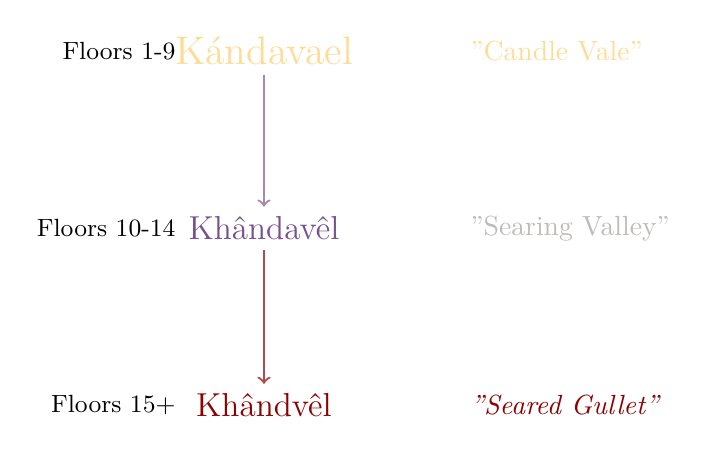
\begin{tikzpicture}[scale=1.5]
    % Phonetic transformation diagram
    \node[dawn, font=\Large\displayfont] (high) at (0,3) {Kándavael};
    \node[dusk, font=\large] (mid) at (0,1.5) {Khândavêl};
    \node[blood, font=\large\runefont] (low) at (0,0) {Khândvêl};
    
    \draw[->, thick, color=corruption!50] (high) -- (mid);
    \draw[->, thick, color=blood!70] (mid) -- (low);
    
    \node[right=2.5cm, dawn] at (high) {"Candle Vale"};
    \node[right=2.5cm, dusk] at (mid) {\fadetext{"Searing Valley"}};
    \node[right=2.5cm, blood] at (low) {\textit{"Seared Gullet"}};
    
    % Floor indicators
    \node[left=1cm, font=\small] at (high) {Floors 1-9};
    \node[left=1cm, font=\small] at (mid) {Floors 10-14};
    \node[left=1cm, font=\small] at (low) {Floors 15+};
\end{tikzpicture}
\end{center}

\section{The Pattern Emerges}

\begin{tcolorbox}[codexbox={Linguistic Observation}]
The same root words exist in both registers, but their meanings transform through pronunciation:

\begin{tabular}{lll}
\textbf{Root} & \textbf{High Vaelic} & \textbf{Under-Vêlth} \\
\hline
K-N-D & kánde (candle) & khênd (sear, burn) \\
V-L & vael (valley) & vêl (gullet, throat) \\
D-L & dael (dawn) & dæl (drain, bleed) \\
S-L & sael (holy) & sæl (skin, hide) \\
\end{tabular}
\end{tcolorbox}

\section{The Trinity Revealed}

\begin{figure}[h]
\centering
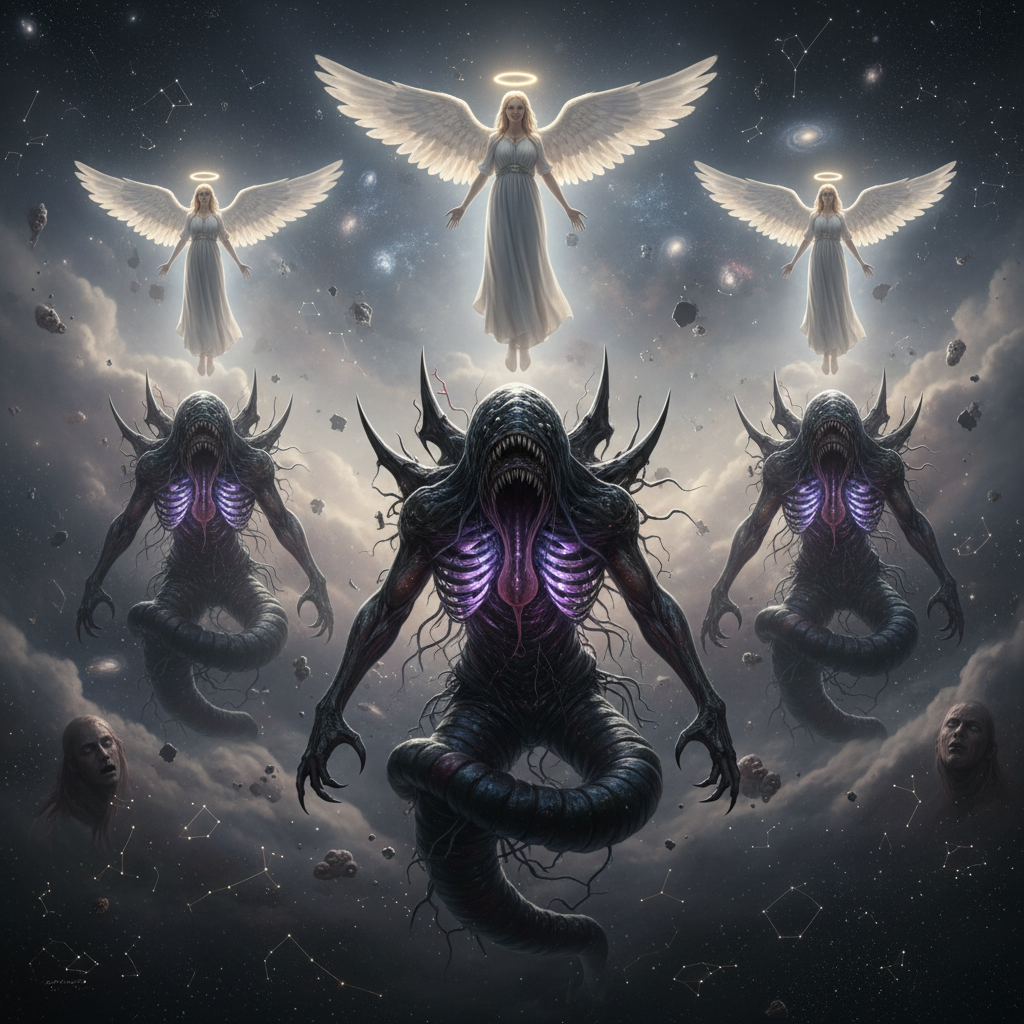
\includegraphics[width=0.8\textwidth]{images/dael_trithae_horror_2025-09-03T22-22-42-860Z_1.png}
\caption*{\textit{The Dael Tríthae... or the Dæl Trith?}}
\end{figure}

\subsection{The Transformation of Prayer}

\begin{adjustwidth}{1em}{1em}
\begin{tabular}{p{2cm}p{4cm}p{4cm}}
\textbf{Floor} & \textbf{Prayer Text} & \textbf{What You Begin to Hear} \\
\hline
1-4 & "Tríthae, breathe on us" & \textit{(sounds normal)} \\
5-9 & "Tríthae, breathe upon us" & \textit{(slightly slurred)} \\
10-14 & "Tríthæ, breathe us" & \textit{(word missing?)} \\
15-19 & "Trithæ, feed on us" & \textit{(surely mishearing)} \\
20+ & "Trith, swallow us" & \textit{(the truth)} \\
\end{tabular}
\end{adjustwidth}

\chapter{The Horror Beneath}

\section{True Nature of the Pantheon}

\begin{tcolorbox}[horrorbox={The Dæl Trith}]
\centering
\runefont\Large
The Three Draining Throats\\
\normalfont
\vspace{1em}
Not gods but \textbf{parasites}. Not divine but \textbf{digestive}.\\
They don't answer prayers—they \textbf{feed on faith}.\\
Every blessing is a \textbf{binding}. Every miracle, a \textbf{meal}.
\end{tcolorbox}

What you thought were three divine tears in their holy symbol are actually three uvulas in waiting throats. The "blessed light" they grant is the phosphorescent glow of decomposition.

\section{The Vardain Truth}

\begin{center}
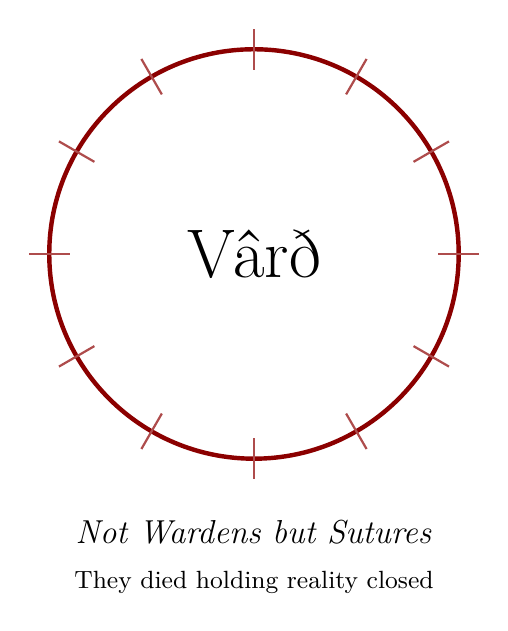
\begin{tikzpicture}[scale=1.3]
    % Draw seal/suture diagram
    \draw[blood, ultra thick] (0,0) circle (2);
    
    % Stitches
    \foreach \angle in {0,30,60,90,120,150,180,210,240,270,300,330} {
        \draw[blood!70, thick] (\angle:1.8) -- (\angle:2.2);
    }
    
    % Central ward symbol
    \node at (0,0) {\Huge\runefont Vârð};
    
    % Labels
    \node[below] at (0,-2.5) {\large\textit{Not Wardens but Sutures}};
    \node[below] at (0,-3) {\small They died holding reality closed};
\end{tikzpicture}
\end{center}

Their death cries, mistranscribed by your "helpful" UI:
\begin{itemize}
    \item "Keep the mob shut!" → \textbf{"Keep the mouth shut!"}
    \item "Hold the dame back!" → \textbf{"Hold the dawn back!"}
    \item "Bar the gait!" → \textbf{"Bar the gate!"}
\end{itemize}

\section{The Corruption of Items}

\subsection{Progressive Revelation Through Description}

\begin{tcolorbox}[itembox={Festival Candle}]
\textbf{Early Game:} \textit{"Hand-dipped beeswax candle. Smells of honey and smoke. A reminder of Kándavael's prosperity."}
\end{tcolorbox}

\begin{tcolorbox}[itembox={Festival Candle}]
\textbf{Mid Game:} \textit{"Long-burning wax for shrine rites. Stabilizes light in windy places. The wick seems... familiar?"}
\end{tcolorbox}

\begin{tcolorbox}[horrorbox={Festival Candle}]
\textbf{Late Game:} \textit{"Rendered tallow, holds clean edge. Whose fat? The wick remembers. It whispers names in Under-Vêlth."}
\end{tcolorbox}

\chapter{The Masks We Wear}

\section{Character Classes as Psychological Horror}

Each "class" represents a different response to the truth, a mask worn to survive the unraveling:

\subsection{The Oathbreaker Knight}

\begin{wrapfigure}{r}{0.35\textwidth}
    \centering
    \begin{tcolorbox}[horrorbox={}, boxrule=2pt, width=\linewidth]
    \textit{"My armor won't come off"}\\
    \vspace{0.5em}
    Once sworn to protect, now the oath protects itself. The blessed plate has fused with flesh, prayer-inscribed metal replacing bone.
    \end{tcolorbox}
\end{wrapfigure}

The Candle Knights' blessing was always a curse. Their armor doesn't protect them—it \textit{replaces} them. Each oath carved into the metal carves away humanity. They can't remove the armor because there's nothing underneath anymore.

\textbf{Abilities:}
\begin{itemize}
    \item \textbf{Fused Aegis}: Damage reduction increases as humanity decreases
    \item \textbf{Oath Scars}: Each broken vow grants power but removes memory
    \item \textbf{Iron Prayer}: Weapons become part of the body permanently
\end{itemize}

\subsection{The Mad Scholar}

\begin{figure}[h]
\centering
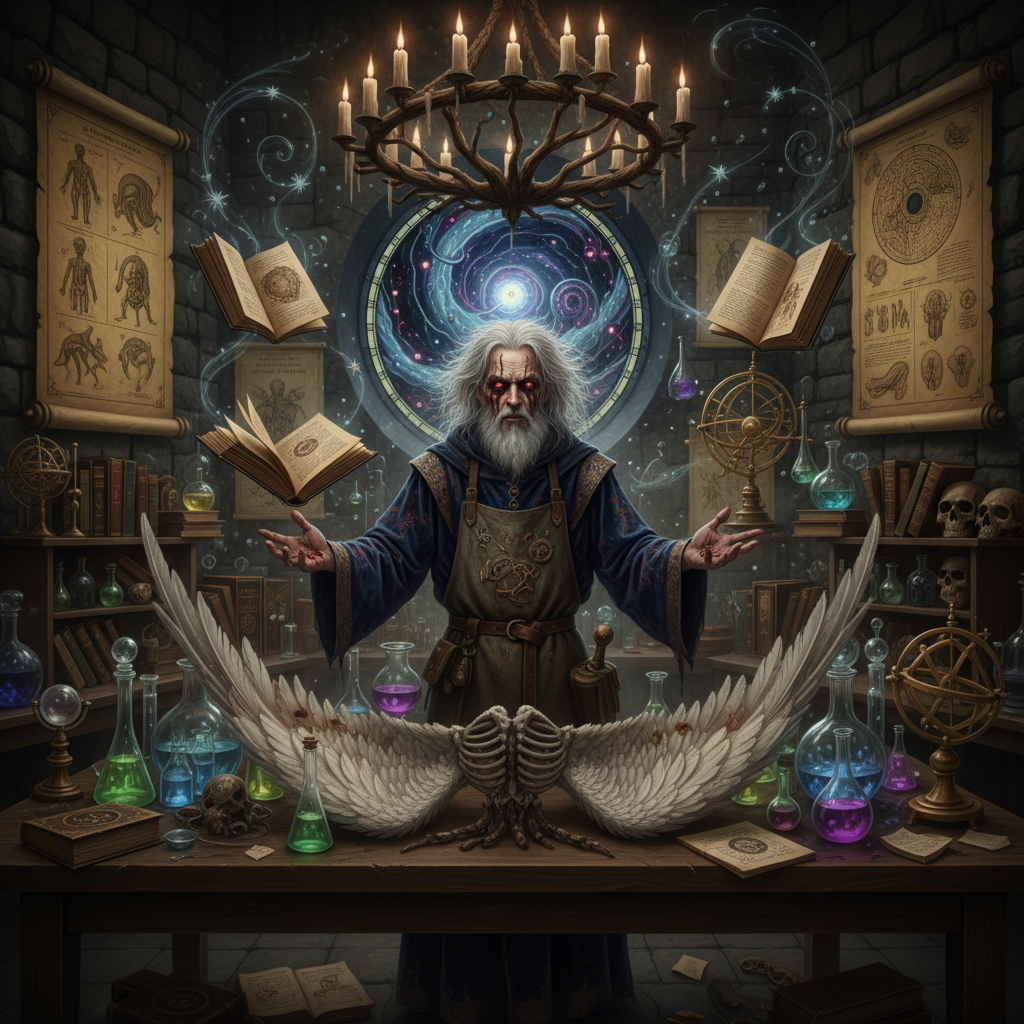
\includegraphics[width=0.7\textwidth]{images/mad_scholar_2025-09-03T22-30-39-545Z_1.png}
\caption*{\textit{The Mad Scholar - eyes that bleed truth}}
\end{figure}

Knowledge is a disease, and you're patient zero. The Anatomical University taught you to dissect reality itself, but some things weren't meant to be understood. Your eyes bleed truth.

\textbf{Abilities:}
\begin{itemize}
    \item \textbf{Void Surgery}: Remove concepts from existence
    \item \textbf{Theoretical Autopsy}: Understand how things died by touching corpses
    \item \textbf{Applied Amnesia}: Forget harmful knowledge to regain sanity
\end{itemize}

\subsection{The Bone Witch}

Every spell costs a finger. Every curse, a tooth. Magic isn't channeled—it's \textit{paid for} in flesh. Your body is currency in the economy of horror.

\subsection{The Plague Engineer}

You brought modern knowledge to a medieval world: gunpowder, antibiotics, the scientific method. But chemistry works \textit{differently} here. Your penicillin breeds new plagues. Your explosives tear holes between realities.

\section{The Anatomical University}

\begin{figure}[h]
\centering
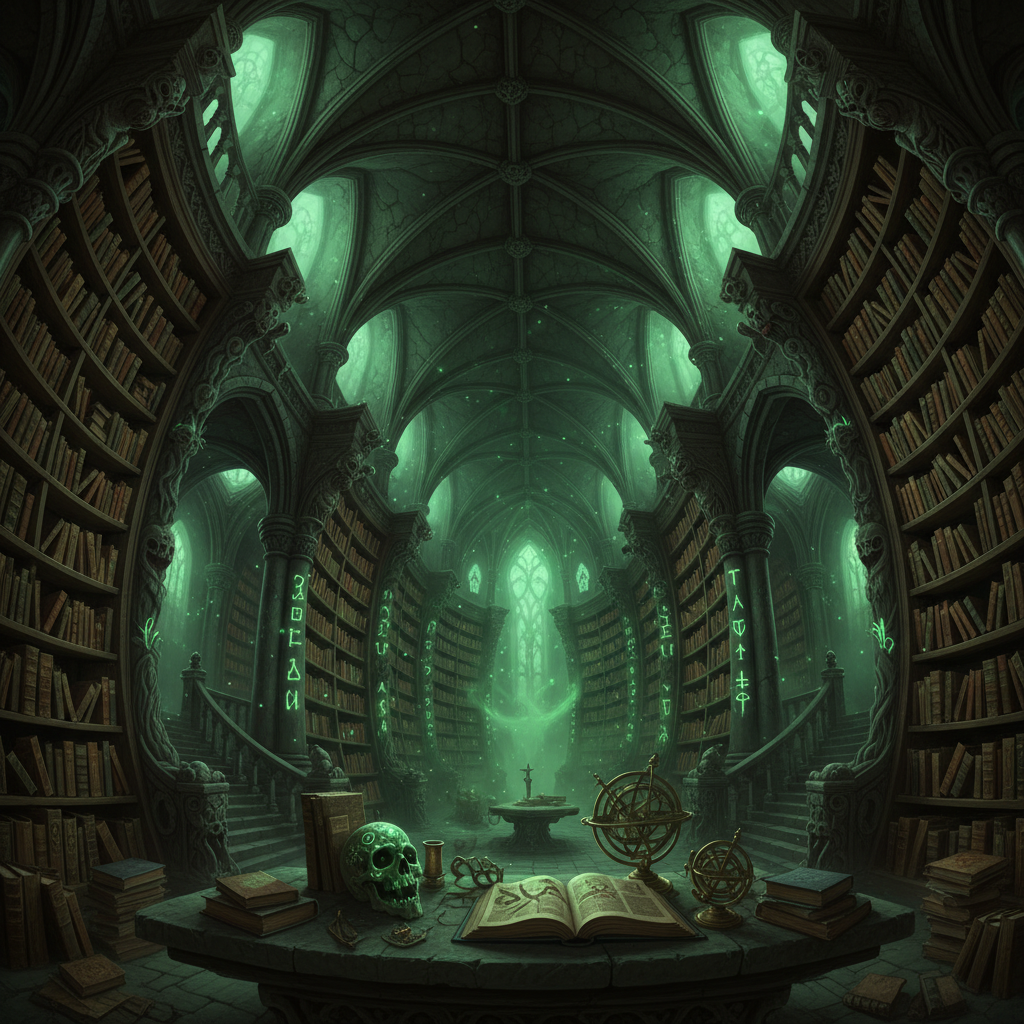
\includegraphics[width=0.8\textwidth]{images/anatomical_university_library_2025-09-03T22-30-07-255Z_1.png}
\caption*{\textit{The Anatomical University Library - where knowledge feeds}}
\end{figure}

A cancer of learning where professors vivisect angels to understand why God went quiet. Students pay tuition in memories and graduate missing organs. The University feeds on curiosity—literally. Each book in the library is bound in the skin of the scholar who wrote it, still warm, still growing hair.

\textbf{Departments:}
\begin{itemize}
    \item \textbf{Void Surgery}: Removing parts of reality that have gone necrotic
    \item \textbf{Theological Autopsy}: Dissecting dead gods to find what killed them
    \item \textbf{Applied Amnesia}: Surgical removal of memories too dangerous to keep
\end{itemize}

\part{The Bestiary of Unmaking}

\chapter{Creatures of the True Layer}

\section{The Listening Worms}

\begin{figure}[h]
\centering
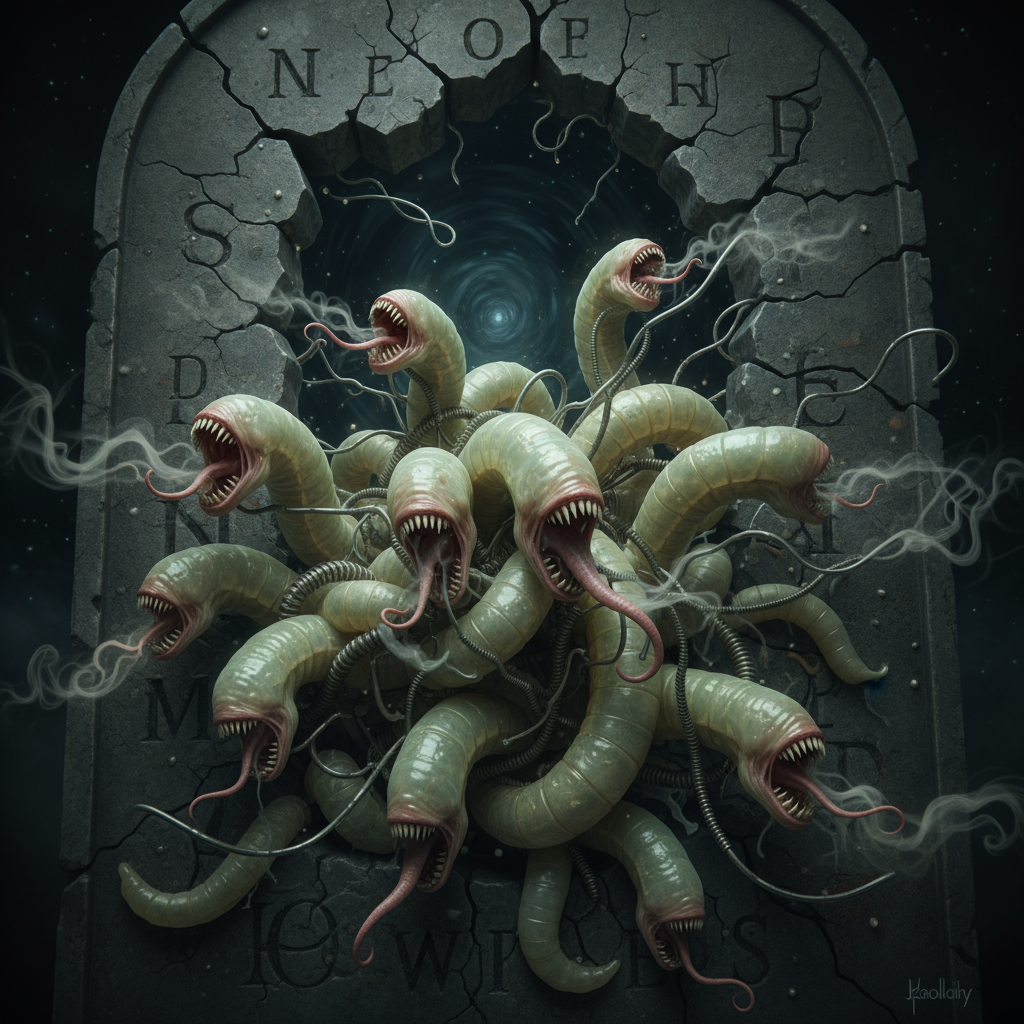
\includegraphics[width=0.7\textwidth]{images/listening_worms_2025-09-03T22-31-43-701Z_1.png}
\caption*{\textit{The Listening Worms - parasites that gestate between words}}
\end{figure}

\begin{tcolorbox}[horrorbox={Paraz'îth Vêl'thar}]
\textit{"They gestate in the space between words"}

Born from lies that were almost true, these parasites don't just mimic voices—they digest them. In darkness, they wear your mother's voice like skin. They speak in the voices of everyone you've failed to save.

\textbf{Behavior:}
\begin{itemize}
    \item Spawn when players tell NPCs false information
    \item Grow stronger near mistranslated text
    \item Drop "Memory Fragments" that contain deleted dialogue
\end{itemize}
\end{tcolorbox}

\section{Corpse Dragons}

\begin{figure}[h]
\centering
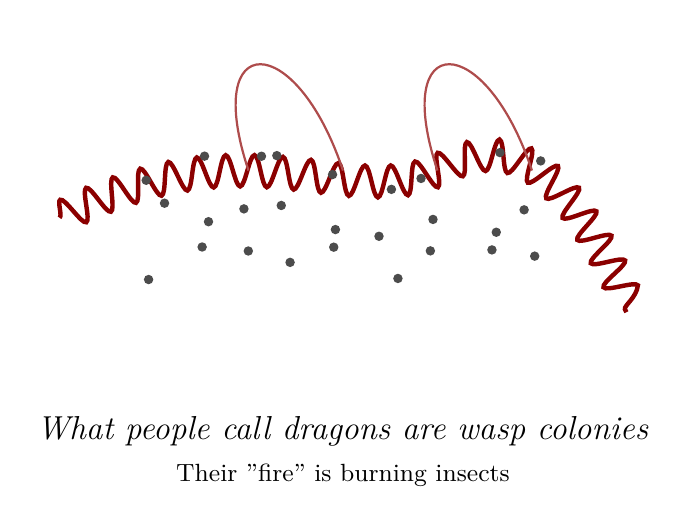
\begin{tikzpicture}[scale=1.2]
    % Dragon outline filled with wasps pattern
    \draw[blood, ultra thick, decorate, decoration={snake, amplitude=2mm}] 
        (0,0) .. controls (2,1) and (3,0) .. (4,0.5) .. controls (5,1) and (5.5,0) .. (6,-1);
    
    % Wings as tattered membranes
    \draw[blood!70, thick] (2,0.5) .. controls (1.5,2) and (2.5,2) .. (3,0.5);
    \draw[blood!70, thick] (4,0.5) .. controls (3.5,2) and (4.5,2) .. (5,0.5);
    
    % Wasp clusters
    \foreach \x in {1,1.5,2,2.5,3,3.5,4,4.5,5} {
        \foreach \y in {-0.5,0,0.5} {
            \fill[black!70] (\x+rand*0.2,\y+rand*0.2) circle (0.05);
        }
    }
    
    \node[below] at (3,-2) {\large\textit{What people call dragons are wasp colonies}}; 
    \node[below] at (3,-2.5) {\small Their "fire" is burning insects};
\end{tikzpicture}
\end{figure}

True dragons died out centuries ago. What remain are their animated corpses, puppeted by colonies of parasitic wasps that nest in brain cavities. Their breath weapon isn't fire—it's billions of burning insects. Their hoards aren't gold—they're mass graves where eggs incubate in human fat.

\begin{figure}[h]
\centering
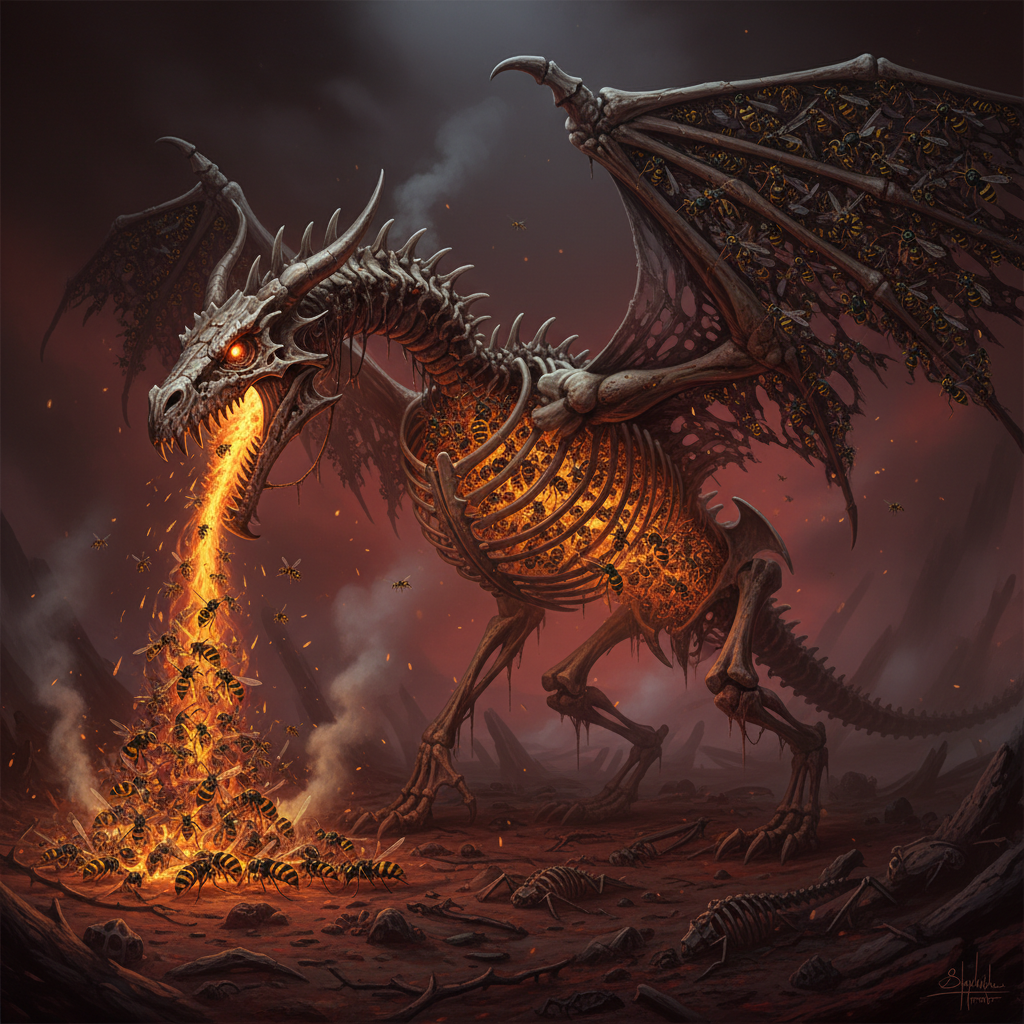
\includegraphics[width=0.75\textwidth]{images/corpse_dragon_2025-09-03T22-30-24-606Z_1.png}
\caption*{\textit{A Corpse Dragon - wasp colonies animating dead wyrm}}
\end{figure}

\section{The Abortion Saints}

\begin{adjustwidth}{1em}{1em}
\textit{People who were retroactively never born, but refuse to stop existing.}
\end{adjustwidth}

Walking paradoxes that reality vomits out continuously. You can't look directly at them—your eyes insist nothing's there while your hands feel cold flesh. They speak in the past tense about futures that won't happen.

\textbf{Combat Mechanics:}
\begin{itemize}
    \item Attacks have a chance to "unhappen"
    \item Killing them erases random memories
    \item They apologize while attacking: "Sorry for not being"
\end{itemize}

\chapter{Locations of Power and Horror}

\section{The Inverse Tower}

\begin{figure}[h]
\centering
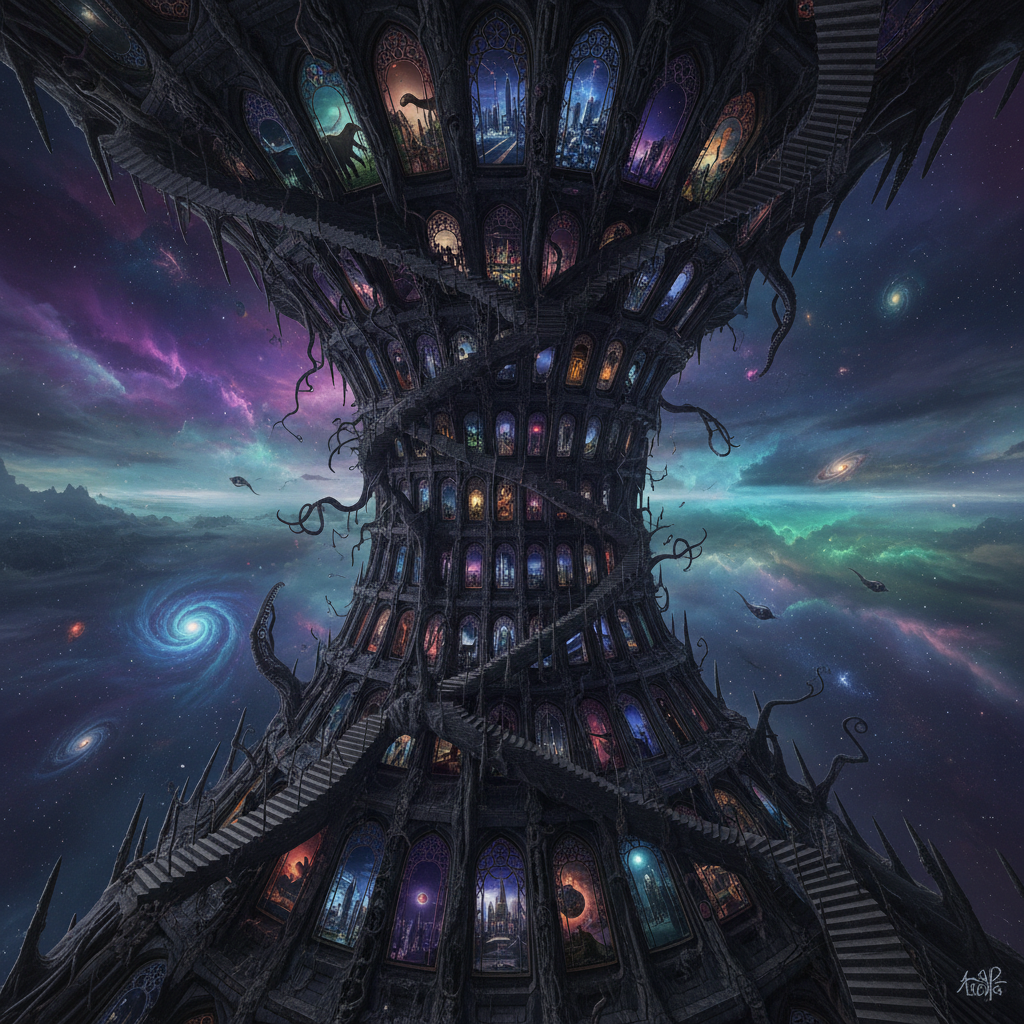
\includegraphics[width=0.8\textwidth]{images/inverse_tower_2025-09-03T22-30-56-469Z_1.png}
\caption*{\textit{The Inverse Tower - where up is down and beginning is end}}
\end{figure}

\begin{center}
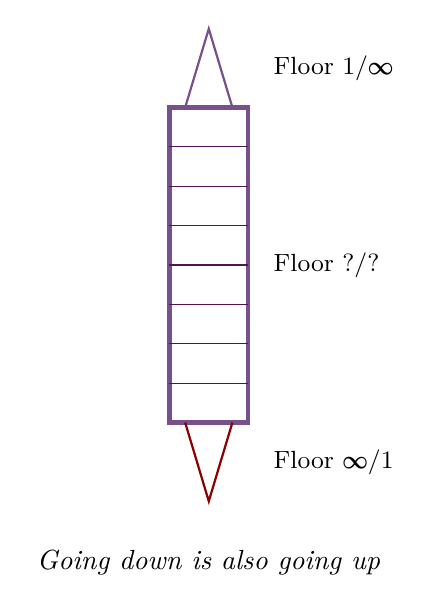
\begin{tikzpicture}[scale=1]
    % Tower extending both ways
    \draw[dusk, ultra thick] (-0.5,2) rectangle (0.5,-2);
    \draw[dusk, thick] (-0.3,2) -- (0,3) -- (0.3,2);
    \draw[blood, thick] (-0.3,-2) -- (0,-3) -- (0.3,-2);
    
    % Floors
    \foreach \y in {1.5,1,0.5,0,-0.5,-1,-1.5} {
        \draw[corruption] (-0.5,\y) -- (0.5,\y);
    }
    
    % Labels
    \node[right] at (0.7,2.5) {\small Floor 1/∞};
    \node[right] at (0.7,0) {\small Floor ?/?};
    \node[right] at (0.7,-2.5) {\small Floor ∞/1};
    
    \node[below] at (0,-3.5) {\textit{Going down is also going up}};
\end{tikzpicture}
\end{center}

A tower that extends downward instead of up, but each floor down is simultaneously a floor up. Mathematically impossible, it exists because no one has successfully disproven it. The bottom floor and top floor are the same room containing both the beginning and end of everything.

\textbf{Notable Features:}
\begin{itemize}
    \item Gravity changes direction based on perception
    \item The library contains books that unwrite themselves
    \item Windows show different timelines of the same view
    \item The stairs remember everyone who never climbed them
\end{itemize}

\section{The Market of Lies}

\begin{figure}[h]
\centering
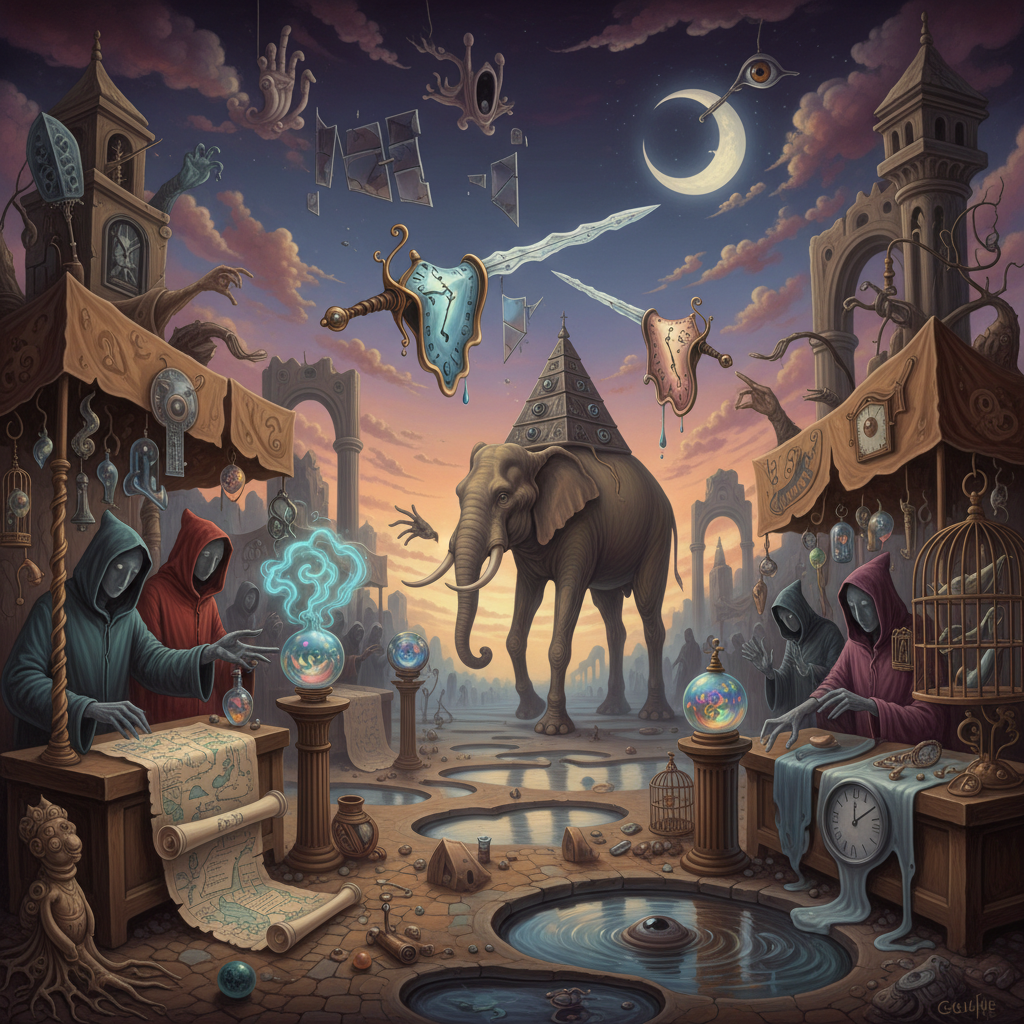
\includegraphics[width=0.75\textwidth]{images/market_of_lies_2025-09-03T22-31-26-965Z_1.png}
\caption*{\textit{The Market of Lies - where false things become real}}
\end{figure}

\begin{tcolorbox}[codexbox={Merchant's Warning}]
\textit{"We sell only what isn't true. But in the True Layer, lies are more solid than facts."}
\end{tcolorbox}

A bazaar where only false things can be sold:
\begin{itemize}
    \item Swords that aren't there (but cut anyway)
    \item Armor that doesn't exist (but stops real blades)  
    \item Maps to nowhere (that lead somewhere worse)
    \item Potions of healing (that heal wounds you haven't received yet)
\end{itemize}

\section{The Garden of Ungrowing}

\begin{figure}[h]
\centering
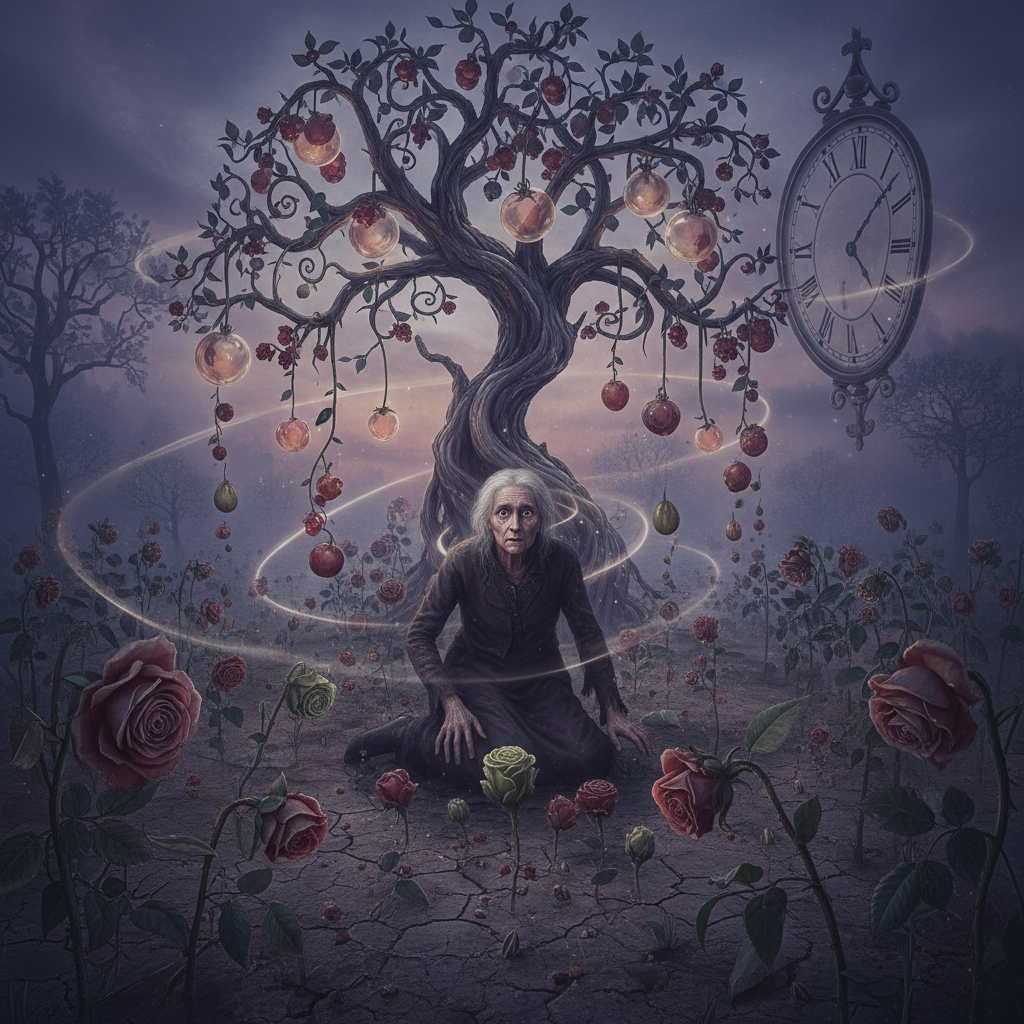
\includegraphics[width=0.8\textwidth]{images/garden_ungrowing_2025-09-03T22-32-01-868Z_1.png}
\caption*{\textit{The Garden of Ungrowing - where time flows backwards}}
\end{figure}

Plants grow backward here, from fruit to seed to nothing. Spend too long and you might ungrow too. The gardener is an old woman getting younger each year, forgetting more of the future daily.

\textit{"I remember when you'll die,"} she says, then forgets she said it.

\part{The Lexicon of Horror}

\chapter{Complete Linguistic Reference}

\section{Phonetic Transformation Rules}

\subsection{The Darkening Process}

\begin{center}
\begin{tabular}{|l|c|c|c|l|}
\hline
\textbf{Stage} & \textbf{High Vaelic} & \textbf{Transitional} & \textbf{Under-Vêlth} & \textbf{Meaning Shift} \\
\hline
Vowels & a /a/ & â /aː/ & â /ɑː/ & bright → dark \\
& ae /eɪ/ & æ /æ/ & a /a/ & diphthong → monophthong \\
& e /e/ & ê /ə/ & ê /ɛ/ & clear → muddy \\
& i /i/ & î /ɪ/ & î /ɪ/ & tense → lax \\
& o /o/ & ô /oː/ & ô /ɔ/ & closed → open \\
& u /u/ & û /ʊ/ & û /ʊ/ & rounded → unrounded \\
\hline
Consonants & l & ll & ɮ & liquid → lateral \\
& r & rh & ʀ & trill → uvular \\
& th /θ/ & ð & t & fricative → stop \\
& k & kh & x & stop → fricative \\
\hline
\end{tabular}
\end{center}

\section{Core Vocabulary}

\subsection{Sacred/Profane Terminology}

\begin{multicols}{2}
\begin{tcolorbox}[heroicbox={High Vaelic}]
\textbf{Religious Terms}\\
\small
\begin{tabular}{ll}
sael-thar & holy water \\
dael-gard & dawn guard \\
rhael-dom & kingdom \\
vael-tríth & valley trinity \\
kánde-lít & candlelight \\
\end{tabular}
\end{tcolorbox}

\columnbreak

\begin{tcolorbox}[horrorbox={Under-Vêlth}]
\textbf{True Meanings}\\
\small
\begin{tabular}{ll}
sæl-thar & skin-render \\
dæl-gard & drain-guard \\
rhal-dom & stitch-dome \\
vêl-trith & throat-three \\
khênd-lît & sear-bright \\
\end{tabular}
\end{tcolorbox}
\end{multicols}

\subsection{Complete Name Registry}

\begin{adjustwidth}{0em}{0em}
\small
\begin{tabularx}{\textwidth}{X|X|X}
\textbf{Entity} & \textbf{High Vaelic} & \textbf{Under-Vêlth} \\
\hline
The Kingdom & Kándavael \textit{"Candle Vale"} & Khândvêl \textit{"Seared Gullet"} \\
The Gods & Dael Tríthae \textit{"Dawn Trinity"} & Dæl Trith \textit{"Draining Throats"} \\
The Villain & Dusk Rhael \textit{"Dusk King"} & Dûšk Rhal \textit{"Twilight Stitcher"} \\
The Guards & Vardain \textit{"Wardens"} & Vârð \textit{"Sutures"} \\
The Priestess & Ael-Saelána \textit{"High-Holy"} & Æl Sælân \textit{"High Flenser"} \\
The Captain & Líndrel \textit{"Line-Leader"} & Lîndrêl \textit{"Cord-Strangler"} \\
The Tower & Daelspire \textit{"Dawn Spire"} & Dælspîr \textit{"Draining Spike"} \\
The Road & Vaelmark \textit{"Vale Mark"} & Vêlmark \textit{"Throat Scar"} \\
The Academy & Saelcairn \textit{"Holy Stones"} & Sælkhairn \textit{"Skin Cairn"} \\
\end{tabularx}
\end{adjustwidth}

\chapter{Lexeme Magic System}

\section{The Language of Reality}

\begin{figure}[h]
\centering
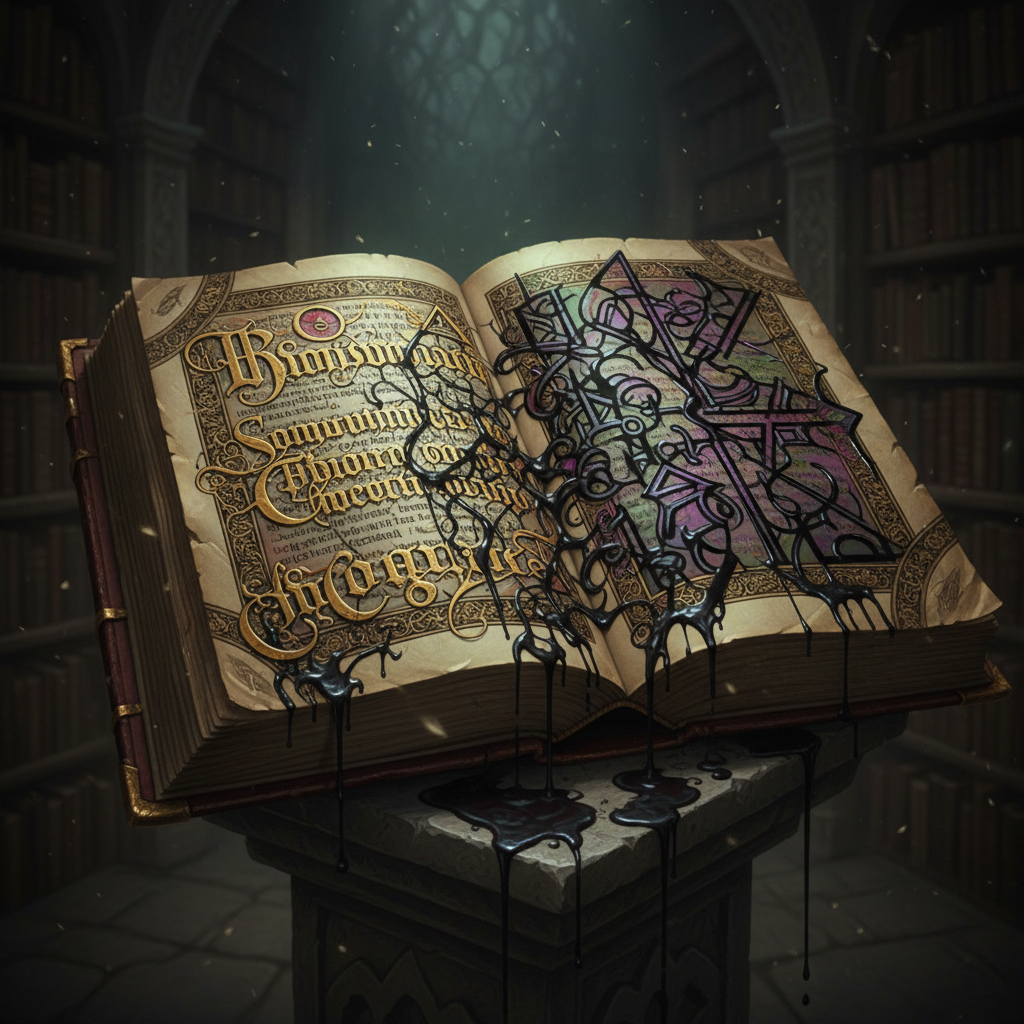
\includegraphics[width=0.7\textwidth]{images/lexeme_tome_2025-09-03T22-22-18-359Z_1.png}
\caption*{\textit{A lexeme tome showing linguistic transformation}}
\end{figure}

Lexemes are the fundamental language spoken by reality itself before consciousness emerged. Each word is a force of nature. Humans weren't meant to speak it—our throats are wrong, our minds too small.

\subsection{Discovery Methods}

\begin{tcolorbox}[codexbox={Acquiring Lexemes}]
\begin{enumerate}
    \item \textbf{Ancient Texts} - Risk: Reading scars the mind permanently
    \item \textbf{Dying Words} - Risk: The speakers might not truly be dying
    \item \textbf{Dream Visions} - Risk: Dreams begin dreaming back into you
    \item \textbf{Herald Teaching} - Risk: Learning spreads their madness
    \item \textbf{Vivisection} - Risk: What you find might still be conscious
\end{enumerate}
\end{tcolorbox}

\subsection{Combination Examples}

\begin{center}
\begin{tabular}{lll}
\textbf{Combination} & \textbf{Effect} & \textbf{Cost} \\
\hline
LIGHT + WARD & Beacon for Them & Increases Notice +5 \\
SELF + HEAL & Burn Tomorrow's Health & Age 1 day per use \\
TIME + REVERSE & Local Causality Break & Sanity -10 \\
TRUTH + SPEAK & Reality Confession & Learn one horrible fact \\
NAME + UN + SELF & Identity Erasure & Become nobody (permanent) \\
\end{tabular}
\end{center}

\section{Forbidden Combinations}

\begin{tcolorbox}[horrorbox={Never Speak These}]
\centering
\textbf{MOUTH + OPEN + ALL}\\
\textit{The Dæl Trith manifest physically}\\
\vspace{0.5em}
\textbf{TRUTH + SEE + ABSOLUTE}\\
\textit{Permanent transition to True Layer}\\
\vspace{0.5em}
\textbf{GOD + UN + MAKE}\\
\textit{Retroactive deity elimination}\\
\end{tcolorbox}

\part{The Meta-Layer}

\chapter{Progressive Revelation Design}

\section{The Five Acts of Descent}

\subsection{Act I: The Golden Age (Floors 1-4)}

\begin{tcolorbox}[heroicbox={Design Principles}]
\begin{itemize}
    \item NO horror elements whatsoever
    \item Cheerful, specific medieval details (bread, smithies, festivals)
    \item Every NPC is helpful and grateful
    \item Combat is against obvious evil (bandits, monsters)
    \item The Dusk King is unambiguously villainous
\end{itemize}
\end{tcolorbox}

\textbf{Forbidden Words in Act I:}
void, writhe, meat, flesh, parasite, cosmic, eldritch, squirm, feed, teeth

\textbf{Required Words in Act I:}
golden, blessed, heroic, noble, dawn, light, hope, peace, prosper

\subsection{Act II: The Shining (Floors 5-9)}

Small oddities with rational explanations:
\begin{itemize}
    \item Prayers answered unusually quickly ("divine favor")
    \item Some items can't be unequipped ("blessed binding")
    \item Villages seem very similar ("traditional architecture")
\end{itemize}

\subsection{Act III: The Cracking (Floors 10-14)}

\begin{itemize}
    \item Language begins shifting in NPC dialogue
    \item Defeated enemies thank you while dying
    \item Your Wisp assistant acts autonomously
    \item Ancient texts show different words than modern ones
\end{itemize}

\subsection{Act IV: The Bleeding (Floors 15-19)}

\begin{itemize}
    \item UI elements corrupt and correct themselves
    \item NPCs speak in mixed registers
    \item Previously killed enemies appear as "allies"
    \item Maps show rooms that weren't there before
\end{itemize}

\subsection{Act V: The Truth (Floor 20+)}

Everything is revealed. The UI admits what it's been hiding. NPCs drop their masks. Your meters show their real names. The true vocabulary unlocks.

\section{Hidden Mechanics}

\subsection{The Three Visible Meters}

\begin{center}
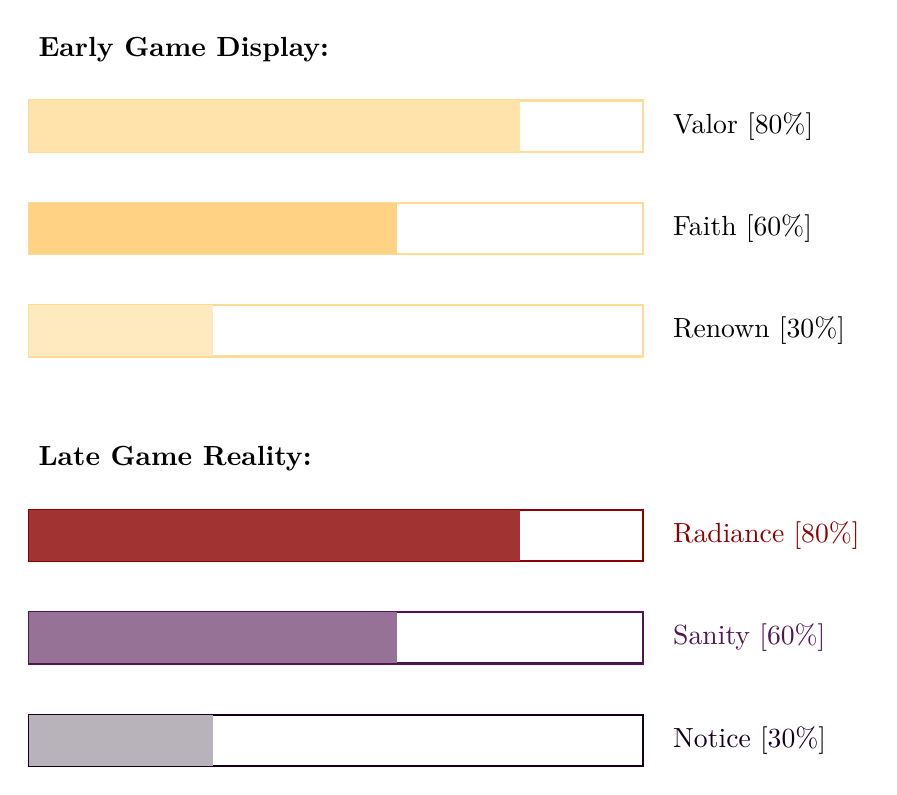
\begin{tikzpicture}[scale=1.3]
    % Early game meters
    \node[anchor=west] at (0,2) {\textbf{Early Game Display:}};
    \draw[dawn, thick] (0,1.5) rectangle (6,1);
    \fill[dawn!80] (0,1.5) rectangle (4.8,1);
    \node[right] at (6.2,1.25) {Valor [80\%]};
    
    \draw[dawn, thick] (0,0.5) rectangle (6,0);
    \fill[candlelight!80] (0,0.5) rectangle (3.6,0);
    \node[right] at (6.2,0.25) {Faith [60\%]};
    
    \draw[dawn, thick] (0,-0.5) rectangle (6,-1);
    \fill[dawn!60] (0,-0.5) rectangle (1.8,-1);
    \node[right] at (6.2,-0.75) {Renown [30\%]};
    
    % Late game revelation
    \node[anchor=west] at (0,-2) {\textbf{Late Game Reality:}};
    \draw[blood, thick] (0,-2.5) rectangle (6,-3);
    \fill[blood!80] (0,-2.5) rectangle (4.8,-3);
    \node[right] at (6.2,-2.75) {\textcolor{blood}{Radiance [80\%]}};
    
    \draw[corruption, thick] (0,-3.5) rectangle (6,-4);
    \fill[corruption!60] (0,-3.5) rectangle (3.6,-4);
    \node[right] at (6.2,-3.75) {\textcolor{corruption}{Sanity [60\%]}};
    
    \draw[void, thick] (0,-4.5) rectangle (6,-5);
    \fill[void!30] (0,-4.5) rectangle (1.8,-5);
    \node[right] at (6.2,-4.75) {\textcolor{void}{Notice [30\%]}};
\end{tikzpicture}
\end{center}

The meters never change mechanically—only your understanding of what they represent changes.

\subsection{Hidden Attention Mechanic}

\begin{tcolorbox}[codexbox={Attention Thresholds}]
\begin{tabular}{ll}
\textbf{Attention Level} & \textbf{Effect} \\
\hline
0-10 & No effect \\
11-25 & Enemies path toward light \\
26-40 & NPCs use titles before names \\
41-60 & Blessed items lock permanently \\
61-80 & Wisp completes unrequested actions \\
81-99 & Reality distortions visible \\
100 & The Dæl Trith manifest \\
\end{tabular}
\end{tcolorbox}

\chapter{Implementation Guidelines}

\section{Text-Based Interface Design}

\subsection{Progressive UI Corruption}

\begin{verbatim}
Early Game:
> look
You stand in the blessed Cathedral of Dawn. Golden light 
streams through stained glass, warming your face.

Mid Game:
> look
You stand in the blessed Cathedral of Dawn. Golden light 
str█ams through stained glass, warming your f█ce.

Late Game:
> look
You stand in the bles█ed Cathedral of D█wn. G█lden light 
stre█ms through st█ined gl█ss, w█rming your fl█sh.
\end{verbatim}

\subsection{Sanity-Affected Display}

\begin{itemize}
    \item \textbf{High Sanity}: Clean text, clear descriptions
    \item \textbf{Medium Sanity}: Occasional character substitutions
    \item \textbf{Low Sanity}: Text shimmers, words replace themselves
    \item \textbf{Zero Sanity}: True Layer descriptions only
\end{itemize}

\section{Easter Eggs and Foreshadowing}

\subsection{The Currency}

Every coin has two sides:
\begin{itemize}
    \item Heads: Three suns (actually three mouths)
    \item Tails: A tree (actually a throat diagram)
\end{itemize}

\subsection{The State Motto}

Appears on banners throughout the game:
\begin{center}
\Large
"Dael Garde, Vael Thríve"\\
\normalsize
\textit{"Dawn guard us, vale thrive"}\\
\vspace{0.5em}
But in Under-Vêlth:\\
\Large
"Dæl Garde, Vêl Thrîv"\\
\normalsize
\textit{"Drain guards us, throat thrives"}
\end{center}

\subsection{Architecture Details}

\begin{itemize}
    \item Doorway arches shaped like uvulas
    \item Decorative swirls that are esophageal diagrams
    \item Three-circle patterns everywhere (mistaken for trinity symbols)
    \item Chandeliers hang like polyps
\end{itemize}

\part{Appendices}

\appendix

\chapter{Complete Pronunciation Guide}

\section{High Vaelic Phonology}

\begin{center}
\begin{tabular}{lll}
\textbf{Letter} & \textbf{IPA} & \textbf{English Approximation} \\
\hline
a & /a/ & "father" \\
ae & /eɪ/ & "day" \\
e & /e/ & "bet" \\
i & /i/ & "meet" \\
o & /o/ & "boat" \\
u & /u/ & "boot" \\
\hline
th & /θ/ & "think" \\
r & /r/ & rolled "r" \\
l & /l/ & "light" \\
v & /v/ & "vine" \\
\end{tabular}
\end{center}

\section{Under-Vêlth Phonology}

\begin{center}
\begin{tabular}{lll}
\textbf{Letter} & \textbf{IPA} & \textbf{Description} \\
\hline
â & /ɑː/ & deep "ah" \\
æ & /æ/ & "cat" \\
ê & /ɛ/ & "bed" \\
î & /ɪ/ & "sit" \\
ô & /ɔ/ & "caught" \\
û & /ʊ/ & "put" \\
\hline
kh & /x/ & "loch" (Scottish) \\
rh & /ʀ/ & uvular trill (French "r") \\
ll & /ɮ/ & lateral fricative \\
ð & /ð/ & "this" \\
\end{tabular}
\end{center}

\chapter{Quick Reference Tables}

\section{Name Transformations at a Glance}

\begin{center}
\small
\begin{tabular}{|l|l|l|}
\hline
\textbf{Early Game} & \textbf{Late Game} & \textbf{True Meaning} \\
\hline
Kándavael & Khândvêl & Candle Vale → Seared Gullet \\
Dael Tríthae & Dæl Trith & Dawn Trinity → Draining Throats \\
Dusk Rhael & Dûšk Rhal & Dusk King → Twilight Stitcher \\
Vardain & Vârð & Wardens → Sutures \\
Ael-Saelána & Æl Sælân & High-Holy → High Flenser \\
Líndrel & Lîndrêl & Line-Leader → Cord-Strangler \\
Daelspire & Dælspîr & Dawn Spire → Draining Spike \\
\hline
\end{tabular}
\end{center}

\section{Lexeme Quick Combinations}

\begin{center}
\begin{tabular}{|l|l|l|}
\hline
\textbf{Input} & \textbf{Output} & \textbf{Hidden Cost} \\
\hline
LIGHT + WARD & Protection & Beacon effect \\
HEAL + SELF & Restoration & Tomorrow's health \\
BLESS + WEAPON & Enhancement & Can't unequip \\
FIRE + SPREAD & Area damage & Attention +3 \\
DARK + HIDE & Invisibility & Sanity -5 \\
TIME + SLOW & Speed boost & Age +1 hour \\
\hline
\end{tabular}
\end{center}

\chapter{Design Philosophy}

\section{Core Principles}

\begin{enumerate}
    \item \textbf{Player Agency Drives Horror}: Every revelation comes from player success, not failure
    \item \textbf{Language Is Gameplay}: Understanding the linguistic shift IS the puzzle
    \item \textbf{Retrospective Clarity}: Second playthrough reveals all clues were always there
    \item \textbf{No Cheap Scares}: Horror emerges from comprehension, not jumpscares
    \item \textbf{The Lie Is Consistent}: The heroic narrative remains internally logical
\end{enumerate}

\section{The Ultimate Twist}

\begin{tcolorbox}[horrorbox={The Final Truth}]
\centering
\Large
You were never the hero.\\
\vspace{0.5em}
\normalsize
You're the infection vector.\\
\vspace{1em}
Every "heroic" action weakened the Vârð's sutures.\\
The Dusk King was trying to save everyone.\\
The Dawn Triumvirate are cosmic parasites.\\
\vspace{1em}
And you've already done too much damage to undo it.
\end{tcolorbox}

\backmatter

\chapter*{Acknowledgments}

\textit{This game explores the horror of language itself—how meaning can corrupt, how understanding can be a curse, and how the words we speak shape the reality we inhabit.}

\vspace{1em}

\textit{In Kándavael, every prayer is a feast, and you're both the supplicant and the meal.}

\vspace{2em}

\begin{center}
\Huge\runefont
Khândvêl Thrîv\\
\normalsize
\vspace{0.5em}
\textit{The Throat Thrives}
\end{center}

\end{document}